\section{Social Affinity filtering}

Affinity filtering is based on the idea that affinity between users
expressed in social networks via interactions and activities is
predictive of user preferences. Figure \ref{Fig1} compares the
accuracies of constant predictor and social matchbox with affinity
filtering (naive bayes, logistic regression and SVM) for interaction
and activity (group, page, favourite) features.

In all of our experiments Affinity filtering performed significantly
better than Social Matchbox and constant predictor except for the
naive bayes.  Naive bayes performed comparatively worse than Logistic
regression and SVM counterpart. It's due to the correlation between
features which is contrary to the conditional independance assumption
made by naive bayes model.

Also, Figure \ref{Fig1} shows that activities are more predictive than
interactions. Among the activities, page likes are the most predictive
followed by group membership and favourites.

%%%%%%%%%%%%%%%%%%%%%%%%%%%%%%%%%%%%%%%%%%%%%%%%%%%%%%%%%%%%%%%%%%%%%%%%%%%
\begin{figure*}[t!]
\centering
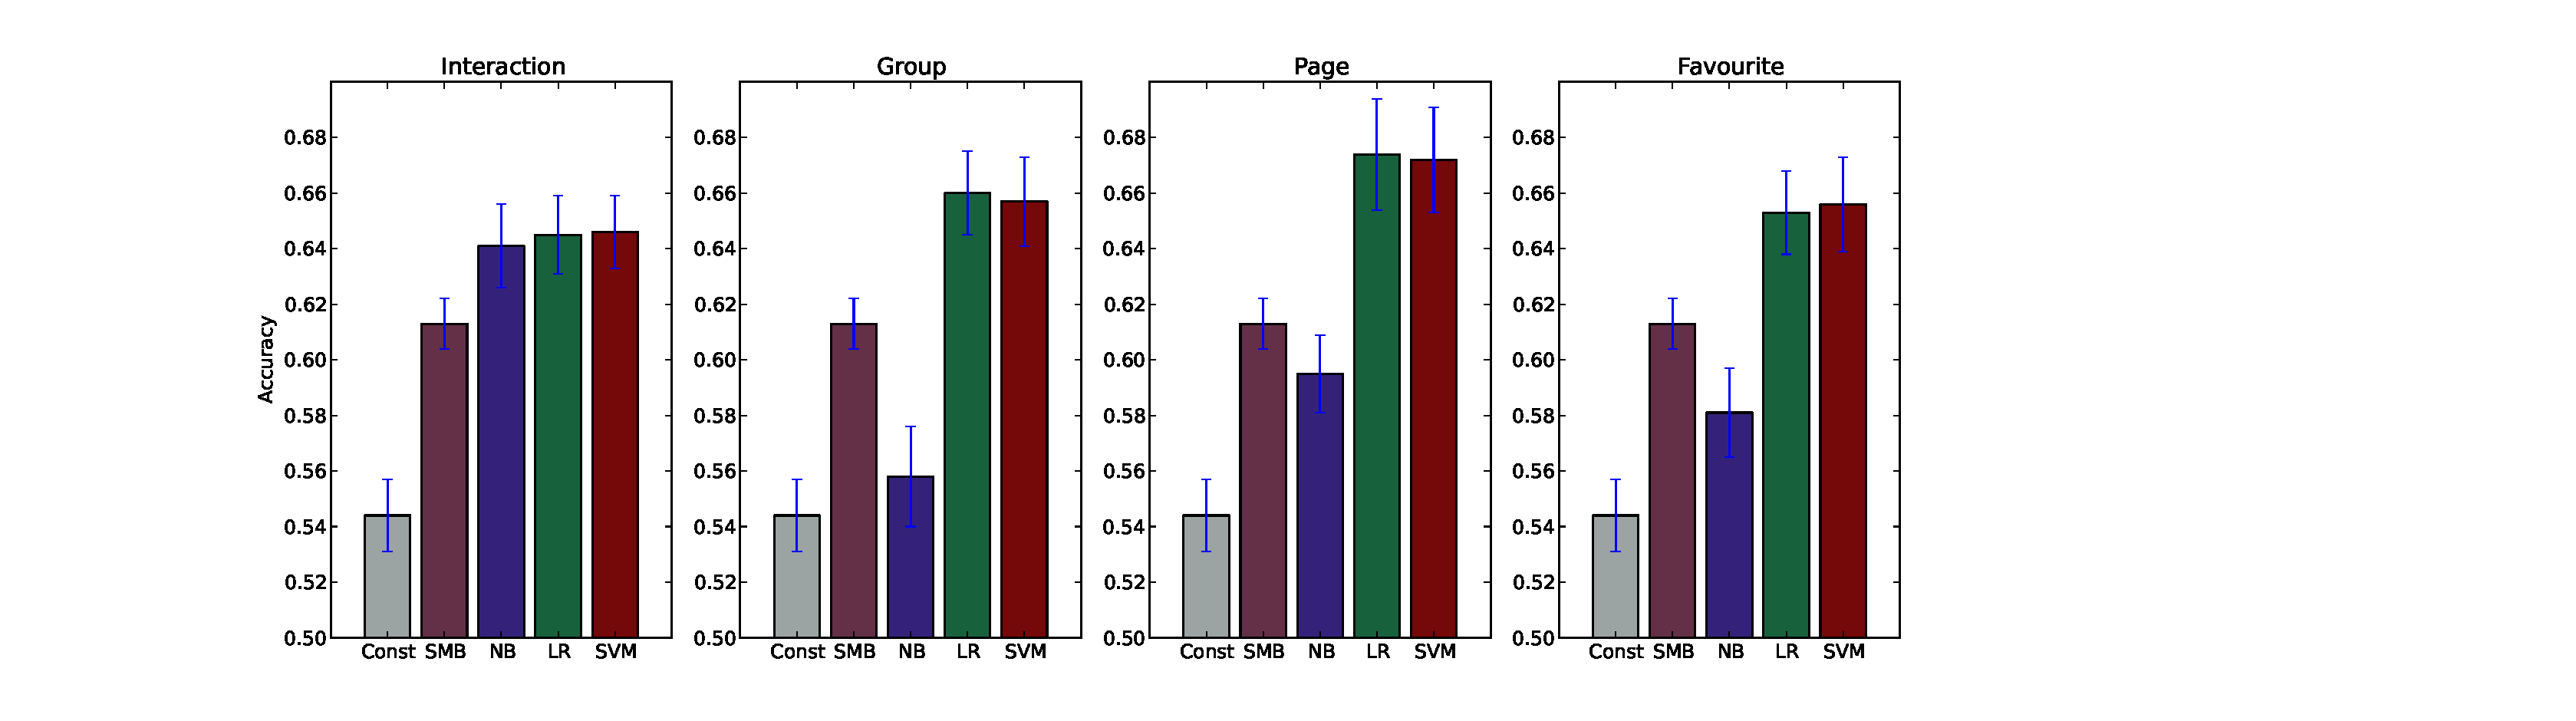
\includegraphics[width=230mm, height=50mm]{data/plots/accuracy/accuracy.eps}
\caption{ Accuracy of predictors (constant, social matchbox, naive bayes, logistic regression, SVM) for Interaction and Activity  features }
\label{Fig1}
\end{figure*}
%%%%%%%%%%%%%%%%%%%%%%%%%%%%%%%%%%%%%%%%%%%%%%%%%%%%%%%%%%%%%%%%%%%%%%%%%%%
